\documentclass[11pt,a4paper]{article}
\usepackage[T1]{fontenc}
\usepackage[utf8]{inputenc}
\usepackage[]{geometry}
\usepackage{afterpage}
\usepackage{tikz}

\usetikzlibrary{fadings}
\definecolor{light}{HTML}{E0E3C2}
\DeclareFixedFont{\titlefont}{T1}{ppl}{b}{n}{1.2cm}
\DeclareFixedFont{\subtitlefont}{T1}{ppl}{m}{n}{0.6cm}
\DeclareFixedFont{\namefont}{T1}{ppl}{m}{n}{0.6cm}
\begin{document}

\afterpage{\restoregeometry}
\newgeometry{left=1in, right=1in,top=1in, bottom=-0.5in}
\definecolor{mytan}{HTML}{1C3651}
\pagecolor{mytan}\afterpage{\nopagecolor}
\thispagestyle{empty}
\begin{center}

\includegraphics{um3.png} \hspace{5em} 
\includegraphics[scale=0.25]{eco.png} \par
\vfill
\titlefont \textcolor{light}{Projet d'économétrie appliquée}\par\vspace{0.5cm}
\subtitlefont \textcolor{light}{Prévision des cours du blé et du nickel}
\vfill
\namefont \textcolor{light}{Mosse Joseph - Rubira Pierre}\par\vspace{0.2cm}
\namefont \textcolor{light}{M1 - MBFA - ARB}
\vfill
\namefont \textcolor{light}{Sous la direction de :}\par\vspace{0.2cm}
\namefont \textcolor{light}{Seyte Françoise}
\end{center}

\begin{center}
\begin{tikzpicture}
\node[scope fading=north, inner sep=0pt, outer sep=0pt]{
 \makebox[\textwidth]{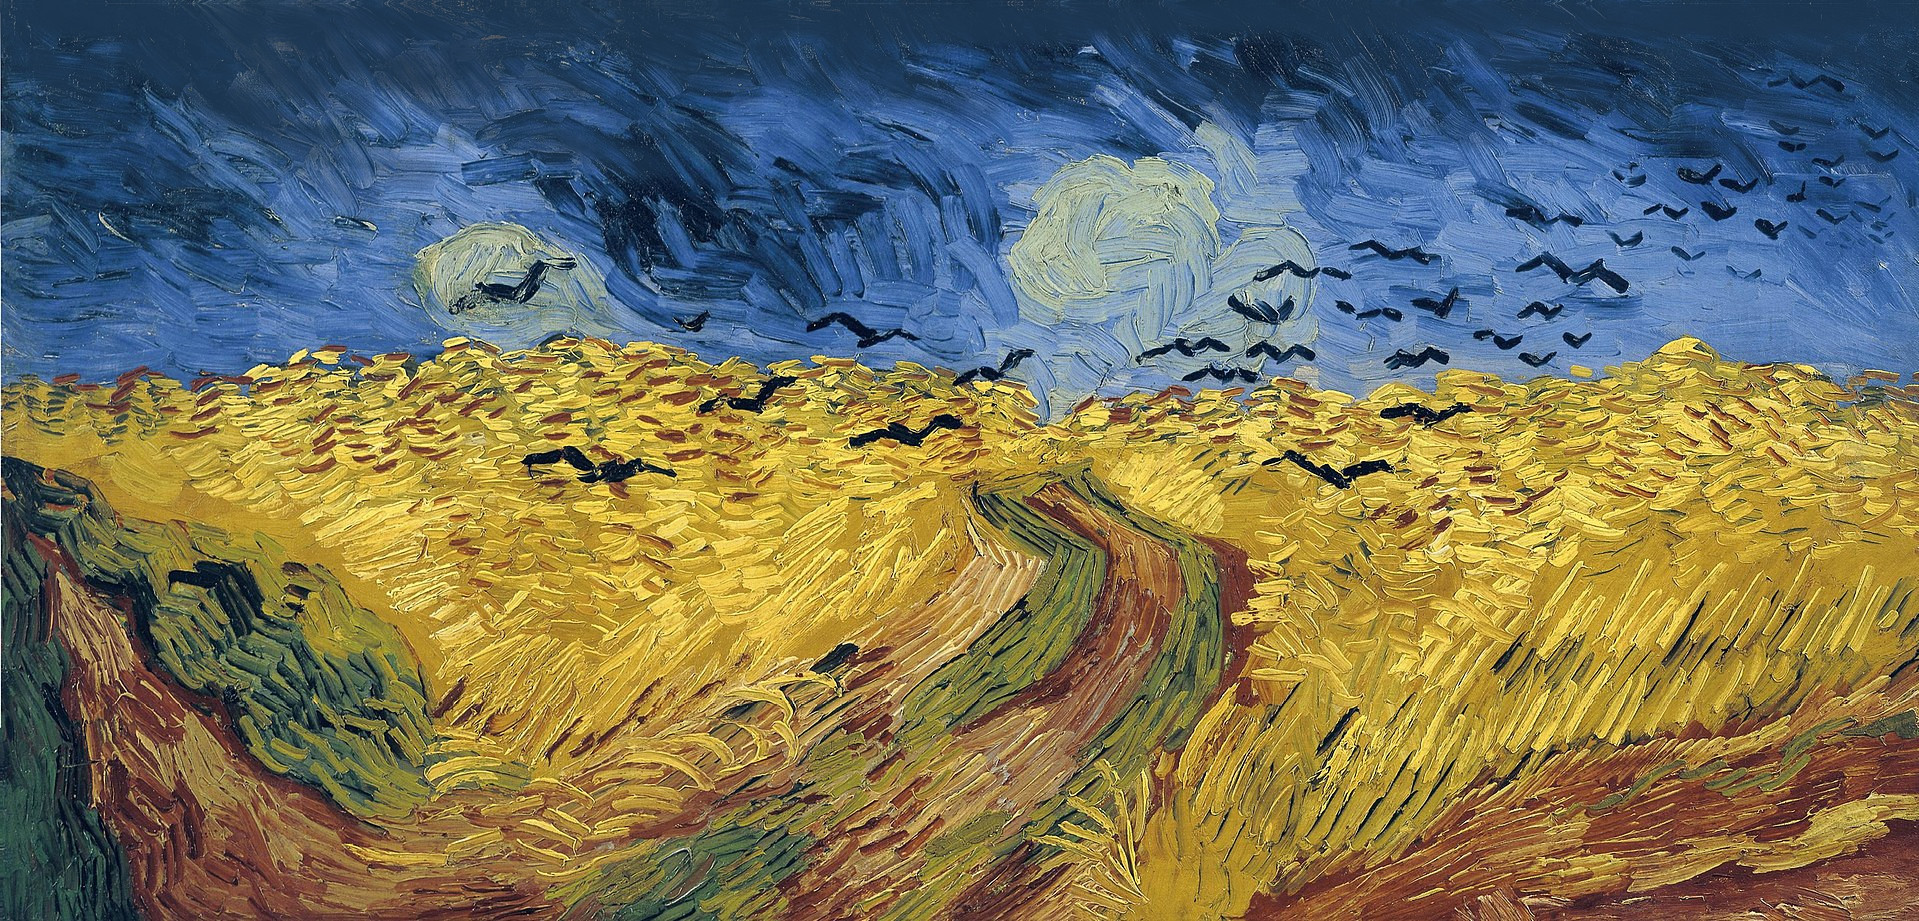
\includegraphics[width=\paperwidth]{ble2.jpg}}
};
\end{tikzpicture}
\end{center}

\clearpage
\setcounter{tocdepth}{1}
\renewcommand\contentsname{Sommaire}
\tableofcontents
\newpage
\section*{Résumé}
\section*{Introduction}
\section{Analyse macroéconomique du blé et du nickel}
\section{Analyse des séries chronologiques}
\section{Prévision par les méthodes traditionnelles}
\section{Prévision selon la méthodologie de Box \& Jenkins}
\section*{Conclusion}






\end{document}